\documentclass[a4paper,12pt]{article} 



%Добавляет возможность искать и копировать текст
\usepackage{cmap}

%Убирает пробел между названием таблицы/рисунка и самой таблицей/рисунком
\usepackage{caption}
\captionsetup[table]{skip= -0 cm}
\captionsetup[figure]{skip= -0 cm}

%Выравнивание названия таблиц по левому краю
%\usepackage[nooneline]{caption} 
%Размеры отступов 
\usepackage[left=20mm, top=20mm, right=20mm, bottom=20mm, footskip=10mm]{geometry}

%Рисунки
\usepackage{graphicx}
\usepackage{wrapfig} %обтекание элементов
\graphicspath{{graphs}{figures}}  % папки с картинками

%Русский язык в формулах
\usepackage{mathtext}

%  Русский язык
\usepackage[T2A]{fontenc}			
\usepackage[utf8]{inputenc}				
\usepackage[english,russian]{babel}	

%Готические буквы
\usepackage{amssymb}

%Знак градусов
\usepackage{gensymb}

% Математика
\usepackage{amsmath,amsfonts,amssymb,amsthm,mathtools} 
\usepackage{wasysym}

%Цветные подписи в таблице
\usepackage[table,xcdraw]{xcolor}

\usepackage{fancyhdr} % Колонтитулы
 	\pagestyle{fancy}
 	\renewcommand{\headrulewidth}{0.3mm}  % Толщина линейки, отчеркивающей верхний колонтитул
 	%\lfoot{Нижний левый}
 	%\rfoot{Нижний правый}
 	\rhead{Белостоцкий Артмемий, Б04-006}
 	%\chead{Верхний в центре}
 	\lhead{Лабораторная работа №4.4.2}
 	% \cfoot{Нижний в центре} % По умолчанию здесь номер страницы
 
\begin{document} 
\begin{titlepage}
	\begin{center}
		\large 	МИНИСТЕРСТВО ОБРАЗОВАНИЯ И НАУКИ РОССИЙСКОЙ ФЕДЕРАЦИИ\\
				МОСКОВСКИЙ ФИЗИКО-ТЕХНИЧЕСКИЙ ИНСТИТУТ \\
				(НАЦИОНАЛЬНЫЙ ИССЛЕДОВАТЕЛЬСКИЙ ИНСТИТУТ)\\ 
				ФИЗТЕХ-ШКОЛА ЭЛЕКТРОНИКИ, ФОТОНИКИ \\
				И МОЛЕКУЛЯРНОЙ ФИЗИКИ \\
		
		
		\vspace{4.0 cm}
		Лабораторная работа № 4.4.2 \\ 
		\LARGE \textbf{Изучение фазовой решетки (эшелет)}
	\end{center}
	\vspace{3 cm} \large
	
	\begin{flushright}
		выполнил студент 2 курса \\
		{группы Б04-006}\\
		\textbf{Белостоцкий Артемий}\\
	\end{flushright}
	
	\vfill

	\begin{center}
	Долгопрудный, 2021 г.
	\end{center}
\end{titlepage}                                                                      
 
\section*{Цель работы} 
 Исследовать спектр ртутной лампы в рабочем порядке и дисперсию эшелета в разных порядках; определить параметры и спектральные характеристики эшелета; оценить влияние ширины пучка на разрешающую способность

\section*{В работе используются}
	\begin{itemize}
		\item гониометр
		\item ртутная лампа
		\item эшелет 
		\item призменный уголковый отражатель 
		\item щель с микрометрическим винтом
	\end{itemize}
 
\section*{Теоретическая часть}
Дифркационная решётка представляет собой стеклянную или металлическую пластину, на которую через строго одинаковые интервалы нанесены параллельные штрихи. Основные параметры дифракционной решётки "--- период $d$ (постоянная решётки), число штрихов $N$.
Условие дифракции Фраунгофера "--- решётка освещается плоской волной, а плоскость наблюдения практически находится в бесконечности.

\begin{figure}[h!]
	\begin{center}
    		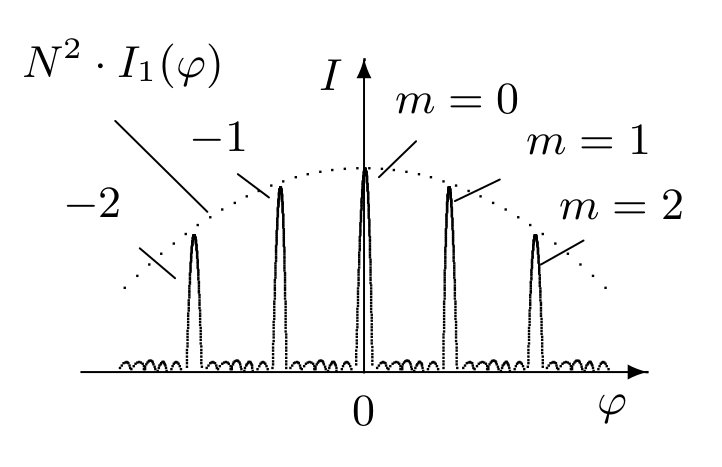
\includegraphics[scale = 0.5]{fig1}
    		\caption{Распределение интенсивности света при дифракции Фраунгофера на решётке}
	\end{center}
\end{figure}
Согласно принципу Гюйгенса-Френеля распределение интенсивности в дифракционной картине определяется суперпозицией волн; амплитуды всех интерферирующих волн при $\varphi$ практически одинаковы; фазы составляют арифметическую прогрессию:
\[
    d \sin \varphi_m = m \lambda,
 \]
 где $m \in Z$ "--- порядок спектра.
 
 Интенсивность $I$ света, распространяющегося под углом $\varphi$ к нормали:
 \[
 I = I_1(\varphi)\frac{\sin^2 (N(dk \sin \varphi) / 2)}{\sin^2 ((dk \sin \varphi) 2)},
 \]
 где $k = \frac{2 \pi}{\lambda}$ "--- волновое число.
 
 Дисперсия $D$ характеризует угловое расстояние между близкими спектральными линиями:
 \[
 D = \frac{d \varphi}{d \lambda} = \frac{m}{d \cos \varphi} = \frac{m}{\sqrt{d^2 - m^2 \lambda^2}}
 \]
 Согласно притерию разрешения Релея, линии становятся неразличимыми, когда расстояние между ними меньше, чем растояние от максимума одной линии до её первого минимума:
 \[
    \frac{Nkd}{2}(\sin (\varphi + \Delta \varphi) - \sin \varphi) = \pi,
 \]
 где $\Delta \varphi$ "--- угловая полуширина главного максимума, $\Delta \varphi = \frac{\lambda}{Nd \cos \varphi}$
 
 
 Разрешающая способность спектрального прибора $R$ вычисляется по формуле:
 \[
 R = \frac{\lambda}{\Delta \lambda} = m \cdot N
 \]
 
\begin{figure}[h]
	\begin{center}
   		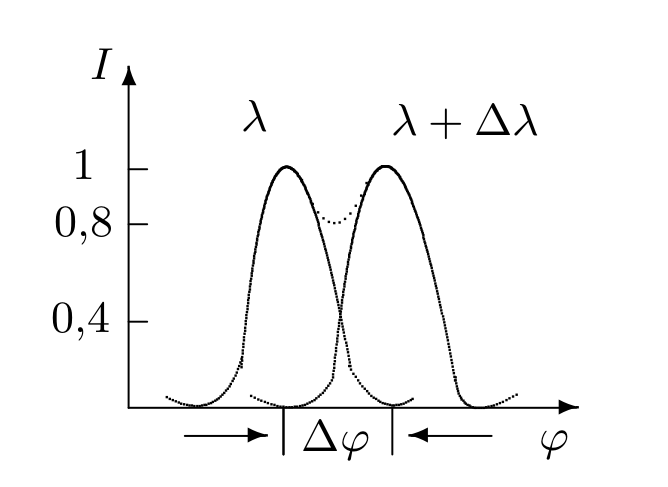
\includegraphics[scale = 0.7]{fig2}
    		\caption{К определению разрешающей способности дифракционной
    		решётки}
		\end{center}
\end{figure}

Дисперсионная область $G$ "--- предельная ширина спектрального интервала $d \lambda$, при которой спектры соседних порядков перекрываются только своими границами:
\[
G = d \lambda = \frac{\lambda}{m}.
\]
 

\section*{Ход работы}
 
\subsubsection*{Исследование спектра ртутной лампы}

Для угла $\psi = 45^o$ измерим угловые координаты спектральных линий ртути в рабочем порядке. Отметим гловую координату каждой из описанных линий:
\begin{table}[h]
	\centering
	\begin{tabular}{|c|c|c|}  \hline
	Ахроматический & $93^o 10' 30''$ & {} \\\hline
	Фиолетовый & $75^o 36' 45''$ & $4047 \dot A$ \\\hline
	Синий & $74^o 23' 45''$ & $4358 \dot A$ \\\hline
	Голубой & $72^o15'35''$ & $4916 \dot A$ \\\hline
 	Зелёный & $70^o12'35''$ & $5461 \dot A$ \\\hline
	Желтый 2 & $69^o 3' 25''$ & $5770 \dot A$ \\\hline
	Жёлтый 1 & $68^o 58'35''$ & $5791 \dot A$ \\\hline
	\end{tabular}
	\end{table}
	Для оценки разрешающей способности измерим гирину одной из линий жёлтого дублета и рассчитаем аппаратную полуширину линии $\Delta \lambda$:
	\[
	\text{Ширина линии:}\ 68^o2'10'' - 68^o2'0'' = 10'' 
	\]
	\[
	\Delta \lambda = \frac{1}{3} \dot A; \quad R = \frac{\lambda}{\Delta \lambda} =\frac{5770}{20} \cdot 60 =  17810
	\]
	Для угла $\psi = 30^o$ измерим координаты каждой из жёлтых линий во всех наблюдаемых порядках:
\begin{table}[h]
\begin{center}
\begin{tabular}{|c|c|c|} \hline
& $Ж_1$ & $89^o3'55''$ \\
\cline{2-3}
$I_{пол}$
& $Ж_2$ & $88^055'45''$ \\\hline
& $Ж_1$ & $39^o50'55''$ \\
\cline{2-3}
$I_{отр}$
& $Ж_2$ & $39^o55'25''$ \\\hline
\end{tabular}
\end{center}
\end{table}
Повторим измерения для $\psi = 45^0, 60^o$:

\begin{table}[h]	
\begin{center}
\begin{tabular}{|c|c|c|} \hline
& $Ж_1$ & $68^058'35''$\\
\cline{2-3}
$I_{отр}$
& $Ж_2$ & $69^o3'35''$ \\\hline
& $Ж_1$ & $48^o32'15''$ \\
\cline{2-3}
$II_{отр}$
& $Ж_2$ & $48^o40'50''$ \\\hline
\end{tabular}
\caption{$\psi = 45^o$}
\end{center}
\end{table}

\begin{table}[h]	
\begin{center}
\begin{tabular}{|c|c|c|} \hline
& $Ж_1$ & $92^o15'5''$\\
\cline{2-3}
$I_{отр}$
& $Ж_2$ & $92^o20'15''$ \\\hline
& $Ж_1$ & $70^o51'45''$ \\
\cline{2-3}
$II_{отр}$
& $Ж_2$ & $71^o0'35''$ \\\hline
& $Ж_1$ & $50^o51'5''$\\
\cline{2-3}
$III_{отр}$
& $Ж_2$ & $51^o4'45''$ \\\hline
\end{tabular}
\caption{$\psi = 60^o$}
\end{center}
\end{table}
\textbf{Зависимость разрешающей силы от ширины пучка:}

Натроим зрительную трубу на желтый дублет в рабочем порядке; определим начало отсчёта "--- момент открытия щели. Крест появляется при $59^o57'20''$; ширина щели "--- 3 деления.

Откроем щель пошире; уменьшая ширину щели, добьемся предельного разрешения желтого дублета, оценим число штрихов:
\[
	 n \approx 1600\ штр/мм; \quad \Delta \lambda = 2 \dot A.
\]
Построим график зависимости $\sin \varphi_m = f(\lambda)$ и по углу наклона определим период эшелета:
\begin{figure}[h]
	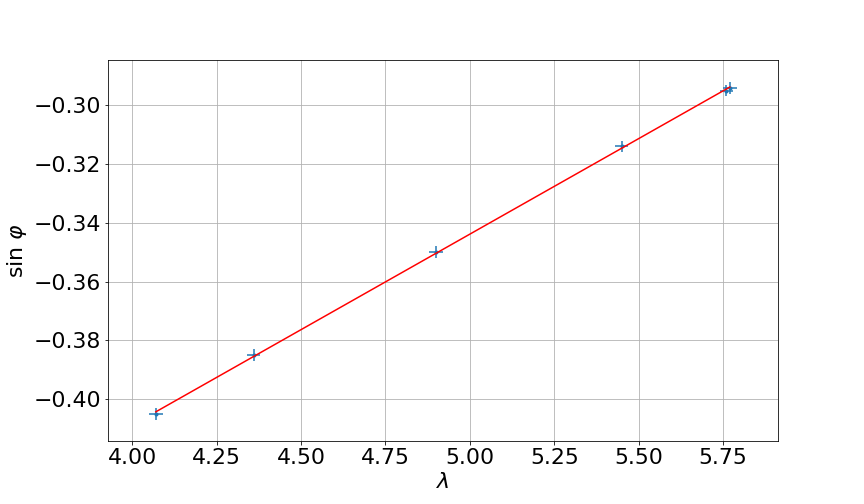
\includegraphics[width = 1.0\linewidth]{g1.png}
	\caption*{Зависимость $\sin \varphi_m$ от $\lambda$}
\end{figure}
Угол наклона графика $k = (6.5 \pm 0.1)\cdot 10^6$

Число штрихов $n \approx 650 \pm 10\ штр/мм$

Период эшелета: $d = \frac{1}{0.65} = 1.53 \pm 0.04$ мм.

Угловая дисперсия в рабочем порядке для жёлтого дублета в угловых секундах на $\dot A$:
\[
D = 14.3\ \frac{угл \cdot сек}{\dot A}
\]
Экспериментальная разрешающая способность:
\[
R = \frac{\lambda}{\Delta \lambda} = 2890
\]
\newpage
\section*{Вывод}
В данной лабораторной работе мы исследовали спектральные характеристики дифракционной решётки, научились работать с гониометром, экспериментально определили период решётки и  разрешающую способность.
\end{document}
 
 
 
 
 
 
 
 
 
 
 
 
 
 
 
 
 
 
 
\end{document}